\chapter{Atividades Desenvolvidas}\label{sec:ativ_desenvolvidas}
Nesta seção, é apresentada, em detalhes, cada uma das principais atividades realizadas para a condução deste projeto.

Ênfase foi dada ao estudo teórico que pudesse embasar o desenvolvimento do aplicativo em si; conceitos como Aprendizagem móvel, Acessibilidade e Usabilidade foram abordados. Além desses, cita-se o estudo teórico das tecnologias utilizadas para a construção do código do aplicativo.

O detalhamento se encontra a seguir:

\section{Estudos sobre usabilidade e acessibilidade}\label{sec:estudos_usab_acess} 

% O que é acessibilidade em termos gerais 
% Em termos digitais (Towards a unified definition of web accessibility. the 12th Web for all Conference, ACM, 2015, p. 35.)

% Falar que alguns softwares e aplicativos impossibilitam o uso de um certo público

% Falar da wcag como uma forma de combater isso
Primeiramente, foram abordados os aspectos relacionados ao conceito de usabilidade bem como a definição de acessibilidade. 

Assim, segundo a Lei 10.098, de 19 de dezembro de 2000 da Legislação Brasileira, a acessibilidade é a possibilidade e condição de alcance para utilização, com segurança e autonomia, dos
espaços, mobiliários e equipamentos urbanos, das
edificações, dos transportes e dos sistemas e meios de comunicação por pessoa portadora de deficiência ou com mobilidade reduzida. Além disso, \cite{torres2002acessibilidade} diz que acessibilidade é um processo dinâmico, associado não só ao desenvolvimento tecnológico, mas principalmente ao desenvolvimento da sociedade. Em geral, está associada a pessoas com deficiências físicas ou psicológicas, idosos ou grupos excluídos; este último mais bem relacionado com o termo \textit{inclusão}. Embora a acessibilidade não se restrinja ao meio digital, é essencial que esteja presente no mesmo. Corroborando com essa ideia, \cite{leew3c} afirma a importância da Web ser utilizável por qualquer um, independente de capacidades individuais ou deficiências. No atual panorama, isso também se aplica ao uso de aplicativos em dispositivos móveis. 

Atrelada à acessibilidade deve estar a usabilidade, que segundo \cite{nielsenPrioritizingWebUsability}
é o atributo relacionado a quão fácil é usar algo. Mais especificamente, refere-se a quão rápido pessoas podem aprender a usar algo, quão eficientes são enquanto o utilizam, quão memorável é, quão propenso a erros e o quanto as pessoas gostam de utilizar; deve-se tornar a utilização fluida. É interessante destacar que existe uma frase entre desenvolvedores que diz: ''não faça o usuário pensar``, com o objetivo de tornar o processo intuitivo o suficiente a ponto de ser considerado natural.
Ainda, é essencial analisar fatores como capacidade de aprendizagem, a fim de que não seja necessário um aprendizado extra por parte do usuário para utilizar o sistema em questão.

% Falar que o problema se aplica a idosos no final da seção
No contexto em que se insere esse projeto isso se torna ainda mais essencial, uma vez que o público idoso sofre bastante com a usabilidade em \textit{smartphones} \citep{dificuldadesIdosos}. Isso ocorre, principalmente, pois investidores da área de tecnologia consideram um grau de incerteza no que tange oportunidades de negócios relacionadas à tecnologia para idosos \citep{NBCelderly}.

Pelo exposto acima, foi decidido seguir recomendações de usabilidade e acessibilidade no desenvolvimento do projeto. É importante ressaltar que o objetivo principal do projeto é auxiliar nos processos de ensino, portanto esse tipo de ação possibilitará que o usuário foque no conteúdo do aplicativo, e não desvie sua atenção por dificuldades de uso.

\section{Estudo sobre Aprendizagem móvel}\label{sec:estudos_ap_movel} 
Outra atividade realizada, foi a abordagem do conceito de aprendizagem móvel bem como uma pesquisa das principais funcionalidades presentes em aplicativos relacionados ao ensino, de palavras cruzadas e relacionados ao idoso.

\subsection{Panorama}
Existem várias definições de \textit{m-learning}. Assim, ao longo dos anos, pesquisadores se dispuseram a estudar o assunto e tentaram achar uma definição. De acordo com \cite{Quinn2000}, \textit{m-learning} é um modelo de aprendizagem eletrônica (\textit{e-learning}) que utiliza equipamentos computadorizados: \textit{Palmtops}, dispositivos que rodam Windows Embedded Compact e até um telefone celular.
Em 2011, \cite{hwang2011research} disseram que uma definição amplamente aceita de \textit{m-learning} é simplesmente ``usar tecnologias móveis para facilitar o aprendizado''. Dentre outras definições, a adotada para esse projeto foi a seguinte: qualquer fornecimento educacional onde a tecnologia dominante é portátil ou dispositivos \textit{palmtop} \citep{traxler2005defining}.

Todavia, independente da definição tomada, torna-se necessário analisar vantagens e desvantagens de utilizar dispositivos móveis. De acordo com \cite{RICHAMEHTA2016} destacam-se como vantagens: 

\begin{itemize}
    \item PDAs ou tablets com anotações e e-books são mais leves e menos volumosos que mochilas cheias de papéis, livros e até laptops;
    \item É mais fácil acomodar dispositivos móveis em uma sala se comparado à computadores de mesa;
    \item Dispositivos móveis podem ser usados em qualquer lugar e em qualquer momento, como em trens, em casa, em hotéis; e isto tem um valor inestimável para a educação \citep{CarmaMaia2008}.
\end{itemize}

Porém, de acordo com \cite{RICHAMEHTA2016}, as seguintes desvantagens devem ser destacadas: 

\begin{itemize}
    \item Celulares pequenos e telas de PDAs limitam-se a quantidade e tipo de informação que pode ser exibida;
    \item Baterias precisam ser recarregadas regularmente, e dados podem ser perdidos caso não se faça o carregamento correto;
    \item É difícil usar gráficos que possuem movimento, especialmente em celulares pequenos.
\end{itemize}
% (i) Celulares pequenos e telas de PDAs limitam-se a quantidade e tipo de informação que pode ser exibida; (ii) Baterias precisam ser recarregadas regularmente, e dados podem ser perdidos caso não se faça o carregamento correto; (iii) É difícil usar gráficos que possuem movimento, especialmente em celulares pequenos.

Dessa forma, devido ao processo de envelhecimento, limitações e desafios podem ser potencializadas no caso de usuários idosos, visto que podem ocorrer mudanças para o idoso durante esse processo. Além disso, é necessário que as aplicações educacionais móveis levem em consideração propostas pedagógicas adequadas e específicas para esse público. Logo, é indispensável que o desenvolvimento dessas aplicações seja realizado de maneira clara e objetiva, possibilitando melhor aprendizagem por parte do idoso.

\subsection{Pesquisa sobre as principais funcionalidades de aplicativos de aprendizagem móvel}
Diversos são os aplicativos que possuem o objetivo de apoiar o processo de ensino e aprendizagem do usuário; seja por meio de jogos, vídeos ou outros materiais. Dessa maneira, alguns aplicativos (para diferentes públicos) foram analisados, a fim de verificar suas funcionalidades e propostas de aprendizagem e acessibilidade, de maneira que essas pudessem ser adaptadas ou utilizadas para aplicações com foco no idoso.

\begin{description}
% Ensina o que? Qual o publico alvo? Pessoas de quantos anos?

\item[Engaging congress]\footnote{\url{https://play.google.com/store/apps/details?id=com.iu.engagingcongress&hl=en}, \url{https://apps.apple.com/us/app/engaging-congress/id1309161238?ls=1}} \hfill \\
\textit{Enganging congress} (\autoref{fig:EngCong}) é um jogo interativo que visa explorar os princípios básicos de um governo representativo. Escolhe-se um tema e é exibido um vídeo. Jogos são incluídos no processo baseados no tema. É importante destacar a atenção dos criadores em fazer o usuário compreender a tarefa; a todo momento é possível clicar no botão de dúvida. As principais funcionalidades são: (i) vídeos educativos sobre o tema; (ii) perguntas relacionadas ao conteúdo passado; (iii) nota final após a conclusão dos exercícios; (iv) botões de dúvidas sempre presentes.

\begin{figure}[ht!]
\centering
    \caption{Telas do aplicativo \textit{Engaging Congress}}
    \label{fig:EngCong}
    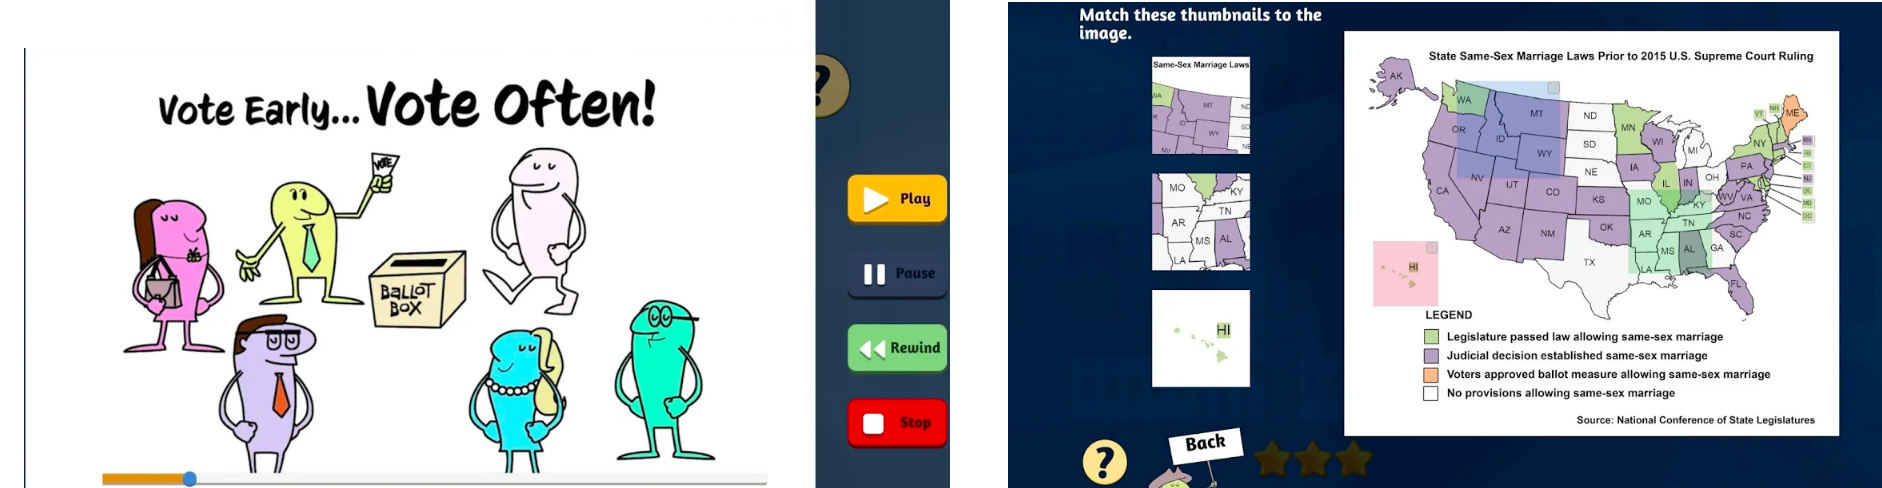
\includegraphics[width=0.9\textwidth]{Figuras/engagingcongress.png}
    
    Fonte: Elaborada pelo autor
\end{figure}

\item[Play PBS KIDS Games]\footnote{\url{https://apps.apple.com/us/app/pbs-kids-games/id1050773989}, \url{https://play.google.com/store/apps/details?id=org.pbskids.gamesapp&hl=pt_BR}} \hfill \\
O aplicativo \textit{Play PBS KIDS Games} (\autoref{fig:pbs}) visa a promoção da educação para crianças na fase de alfabetização (2 a 8 anos), pois contém mais de 100 mini-jogos voltados para tal. As crianças são encorajadas a resolver desafios e aprimorar suas habilidades em ciências, matemática, letras e criatividade. O objetivo é impactar positivamente as vidas de crianças por meio de mídia baseada em um currículo onde quer que elas estejam. O aplicativo ganhou duas premiações no ano de 2017, a saber Melhor aplicativo de jogos para Pré-Escola (\textit{Kidscreen Award Winner}) e o \textit{Parents' Choice Recommended Mobile App}. Os principais recursos são: (i) funcionamento offline; (ii) possibilidade de gerenciar a quantidade de memória que será consumida; (iii) obter detalhes sobre desenhos da TV PBS Kids como idade recomendada e objetivos de aprendizado para as crianças.

\begin{figure}[H]
\centering
    \caption{Telas do aplicativo \textit{Play PBS KIDS Games}}
    \label{fig:pbs}
    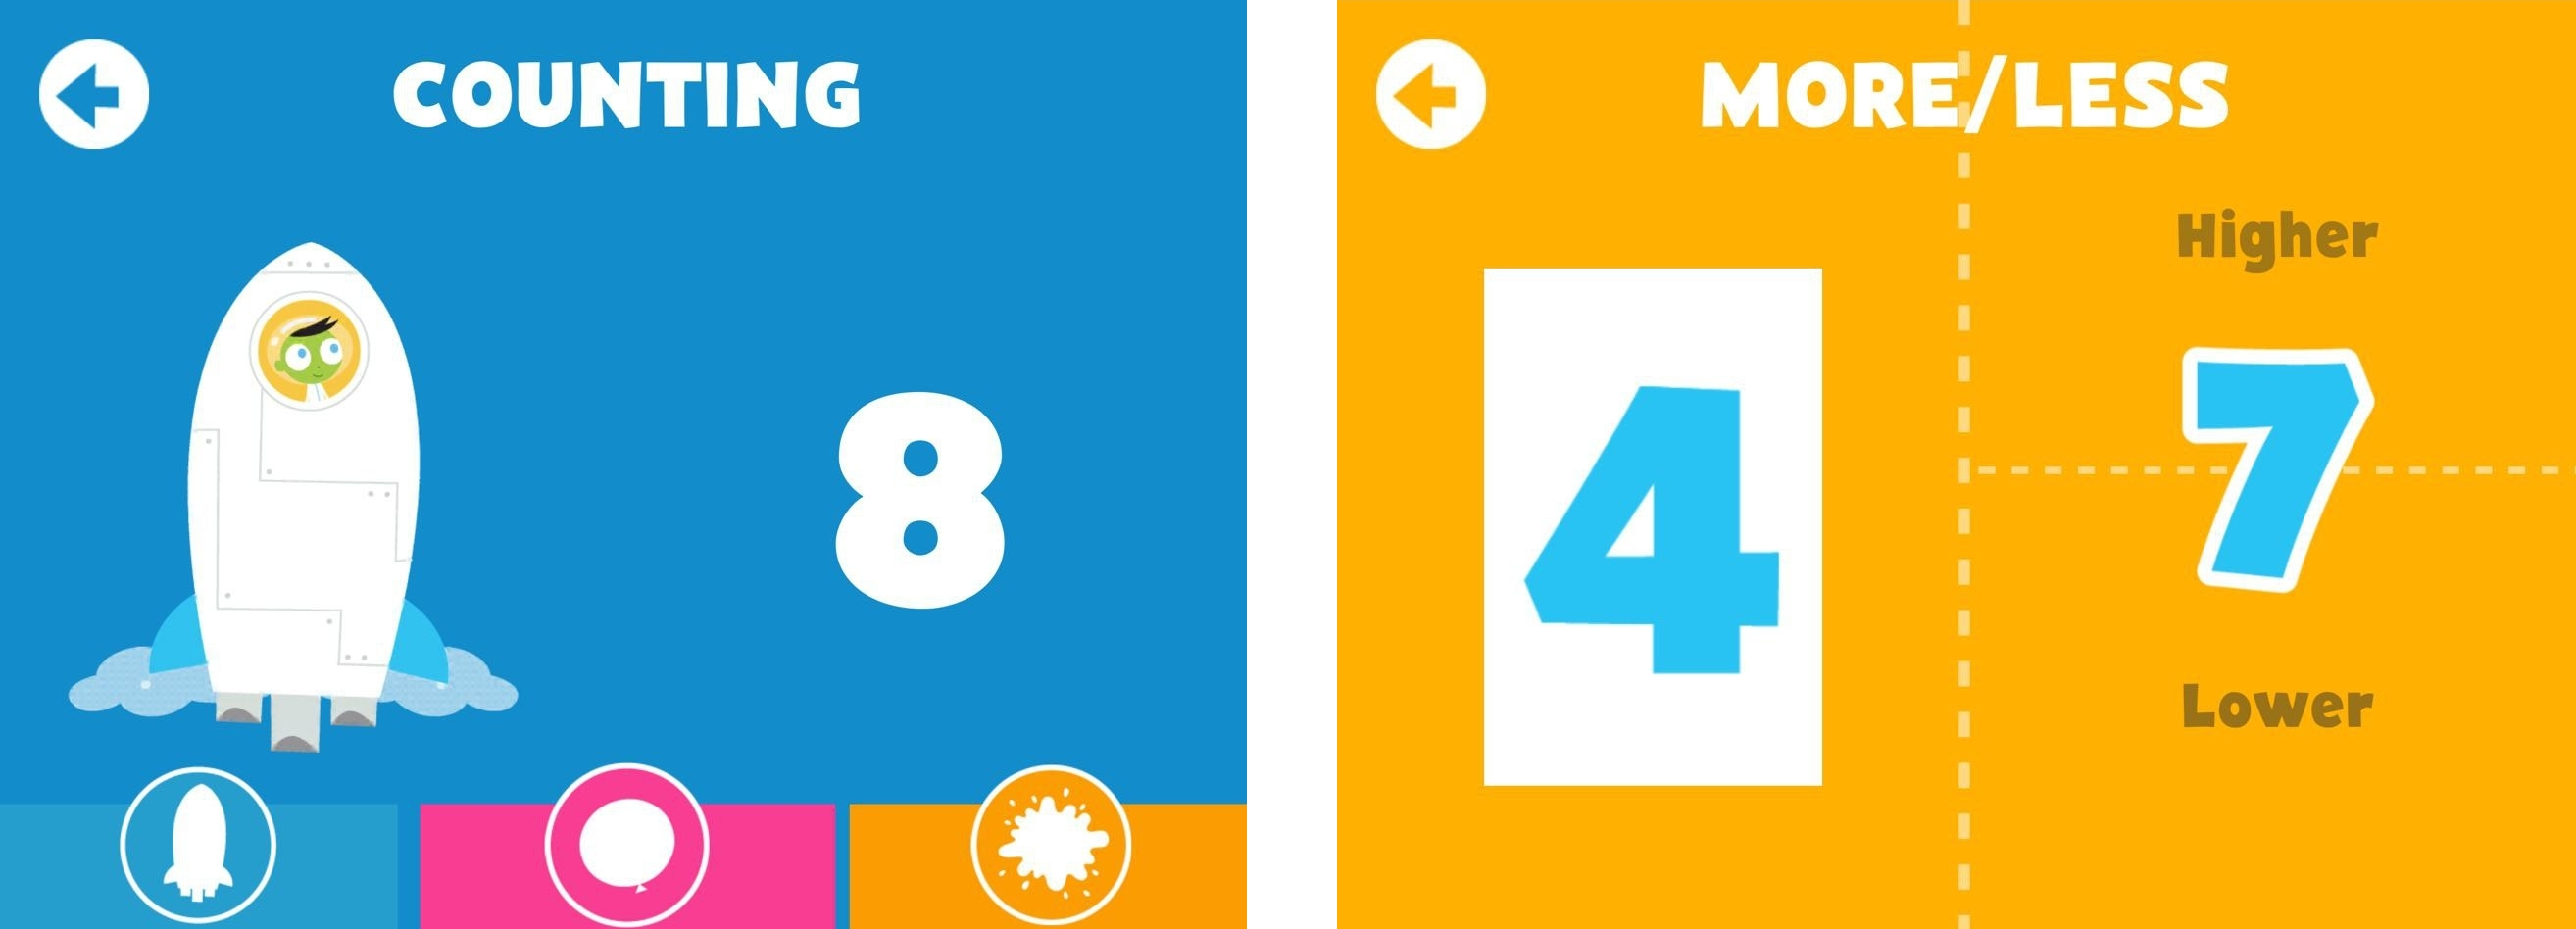
\includegraphics[width=0.9\textwidth]{Figuras/pbsKids.jpg}
    
    Fonte: Elaborada pelo autor
\end{figure}

\item[Human Anatomy Atlas]\footnote{\url{https://apps.apple.com/br/app/human-anatomy-atlas-2020/id1117998129}, \url{https://play.google.com/store/apps/details?id=com.argosy.vbandroid&hl=pt_BR}} \hfill \\
O \textit{Human Anatomy Atlas} (\autoref{fig:humAtlas}) é um aplicativo criado por um time de especialistas em visualização biomédica. É direcionado ao ensino da anatomia do corpo humano com o foco em estudantes e professores, apesar de também ser utilizado em hospitais. Seus modelos em 3D promovem uma fidelidade às estruturas humanas reais, sendo possível rotacionar e dissecar órgãos e partes do corpo. Possui recursos como : (i) interatividade com estruturas 3D; (ii) mais de 1000 questões para testes em assuntos; (iii) visualização de anatomias complexas em realidade aumentada; (iv) disponibilidade em 7 idiomas.

\begin{figure}[ht!]
\centering
    \caption{Telas do aplicativo \textit{Human Anatomy Atlas}}
    \label{fig:humAtlas}
    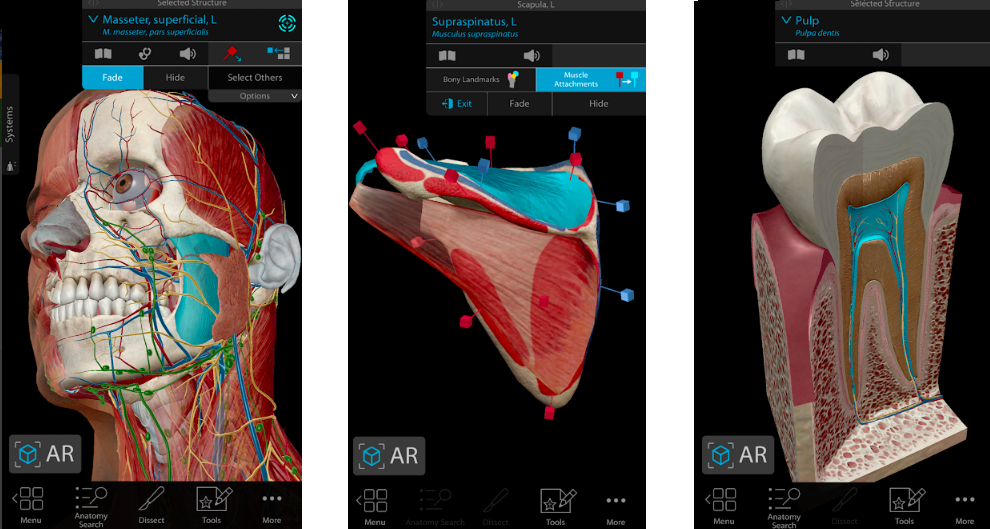
\includegraphics[width=0.9\textwidth]{Figuras/humanAtlas.png}
    
    Fonte: \cite{HumanAnatomyAtlas}
\end{figure}

\item[Bini Super ABC]\footnote{\url{https://apps.apple.com/br/app/bini-abc-alfabeto-crianças-app/id1397966958}, \url{https://play.google.com/store/apps/details?id=com.binibambini.abc&hl=pt_BR}} \hfill \\
Bini Super ABC (\autoref{fig:biniABC}) é um aplicativo voltado para crianças na faixa de 3 a 5 anos na fase de instrução educacional. O aplicativo promove o aprendizado das letras do alfabeto com diversos jogos infantis. O objetivo é tornar o ensino interessante e empolgante com desenhos coloridos, personagens e efeitos sonoros. A aplicação possui as funcionalidades: (i) aprendizado das letras por sons; (ii) reforço do material aprendido; (iii) controle de responsáveis para os jogos.

\begin{figure}[H]
\centering
    \caption{Telas do aplicativo \textit{Bini Super ABC}}
    \label{fig:biniABC}
    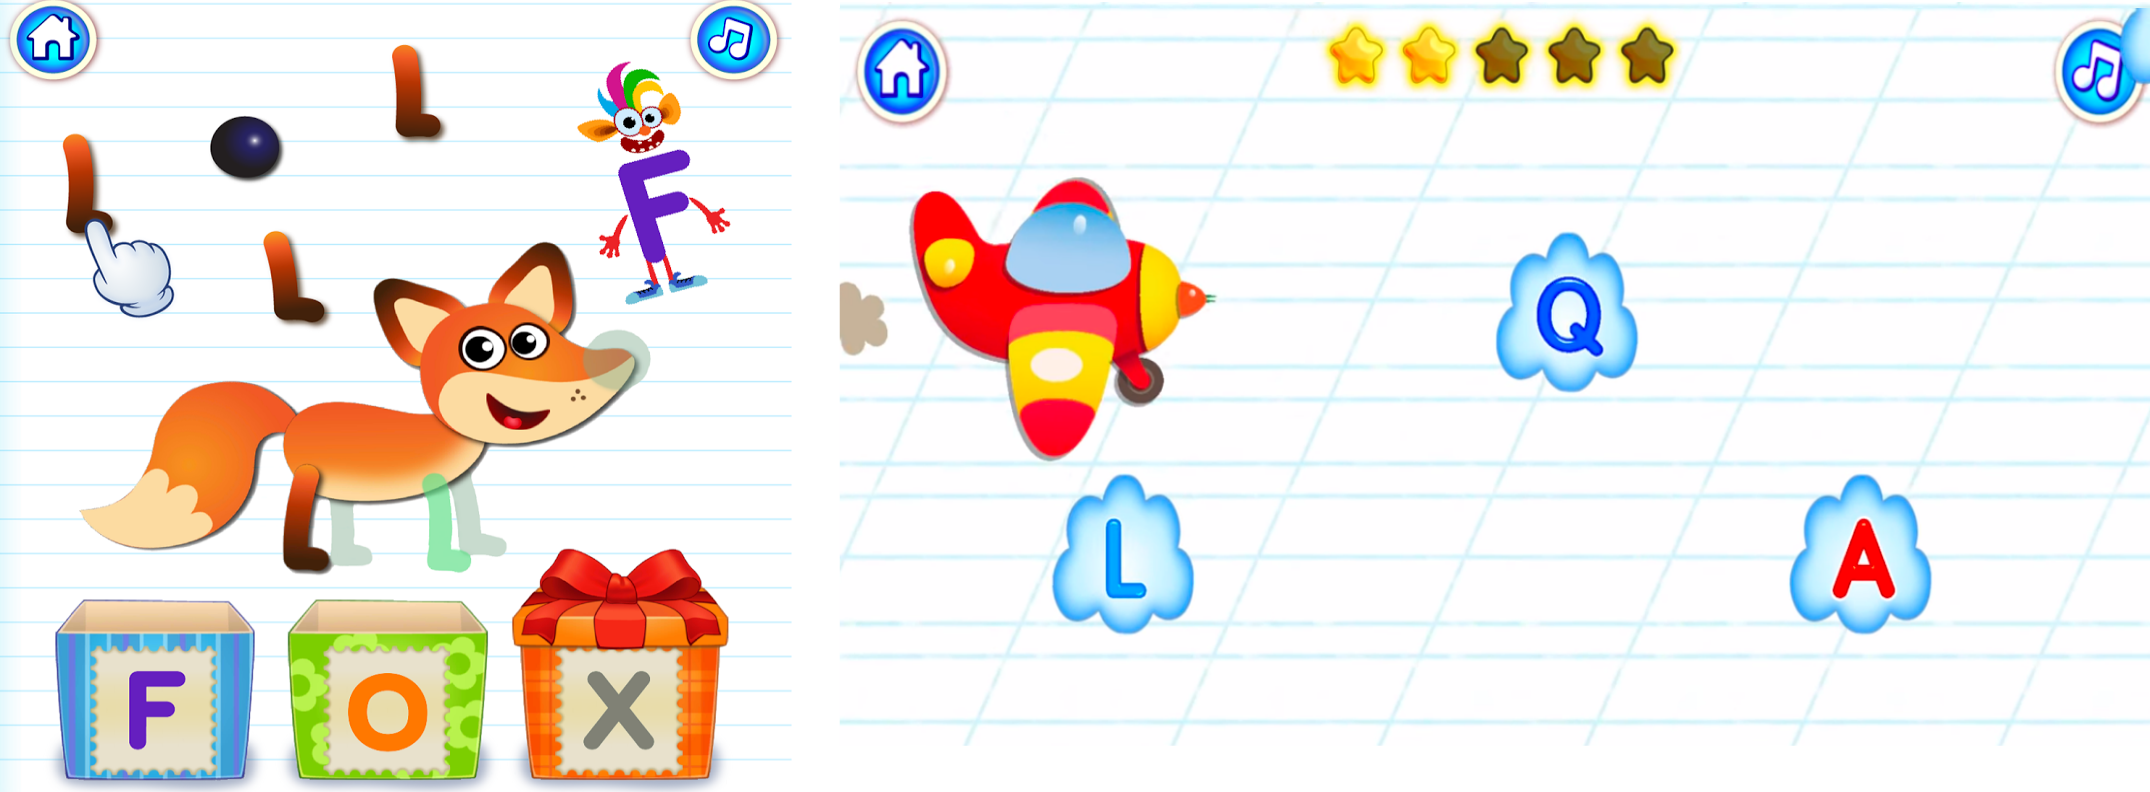
\includegraphics[width=0.9\textwidth]{Figuras/biniabc.png}
    
    Fonte: Elaborada pelo autor
\end{figure}

\item[Crossword Puzzle Free]\footnote{\url{https://play.google.com/store/apps/details?id=mobi.redstonegames.crossword.en&hl=pt_BR}} \hfill \\
Crossword Puzzle Free (\autoref{fig:crossFree}) é um aplicativo de palavras cruzadas. É de fácil  uso por não exigir conhecimentos específicos do usuário. Com os 4 níveis de dificuldade é possível buscar o desafio na medida certa além de motivar o usuário a continuar utilizando o aplicativo por não ser nem muito fácil nem muito difícil. As principais funcionalidade são: (i) Teclado do próprio aplicativo; (ii) Dicas aparecem acima do teclado; (iii) Botão de dica para a palavra.


\begin{figure}[H]
\centering
    \caption{Telas do aplicativo \textit{Crossword Puzzle Free}}
    \label{fig:crossFree}
    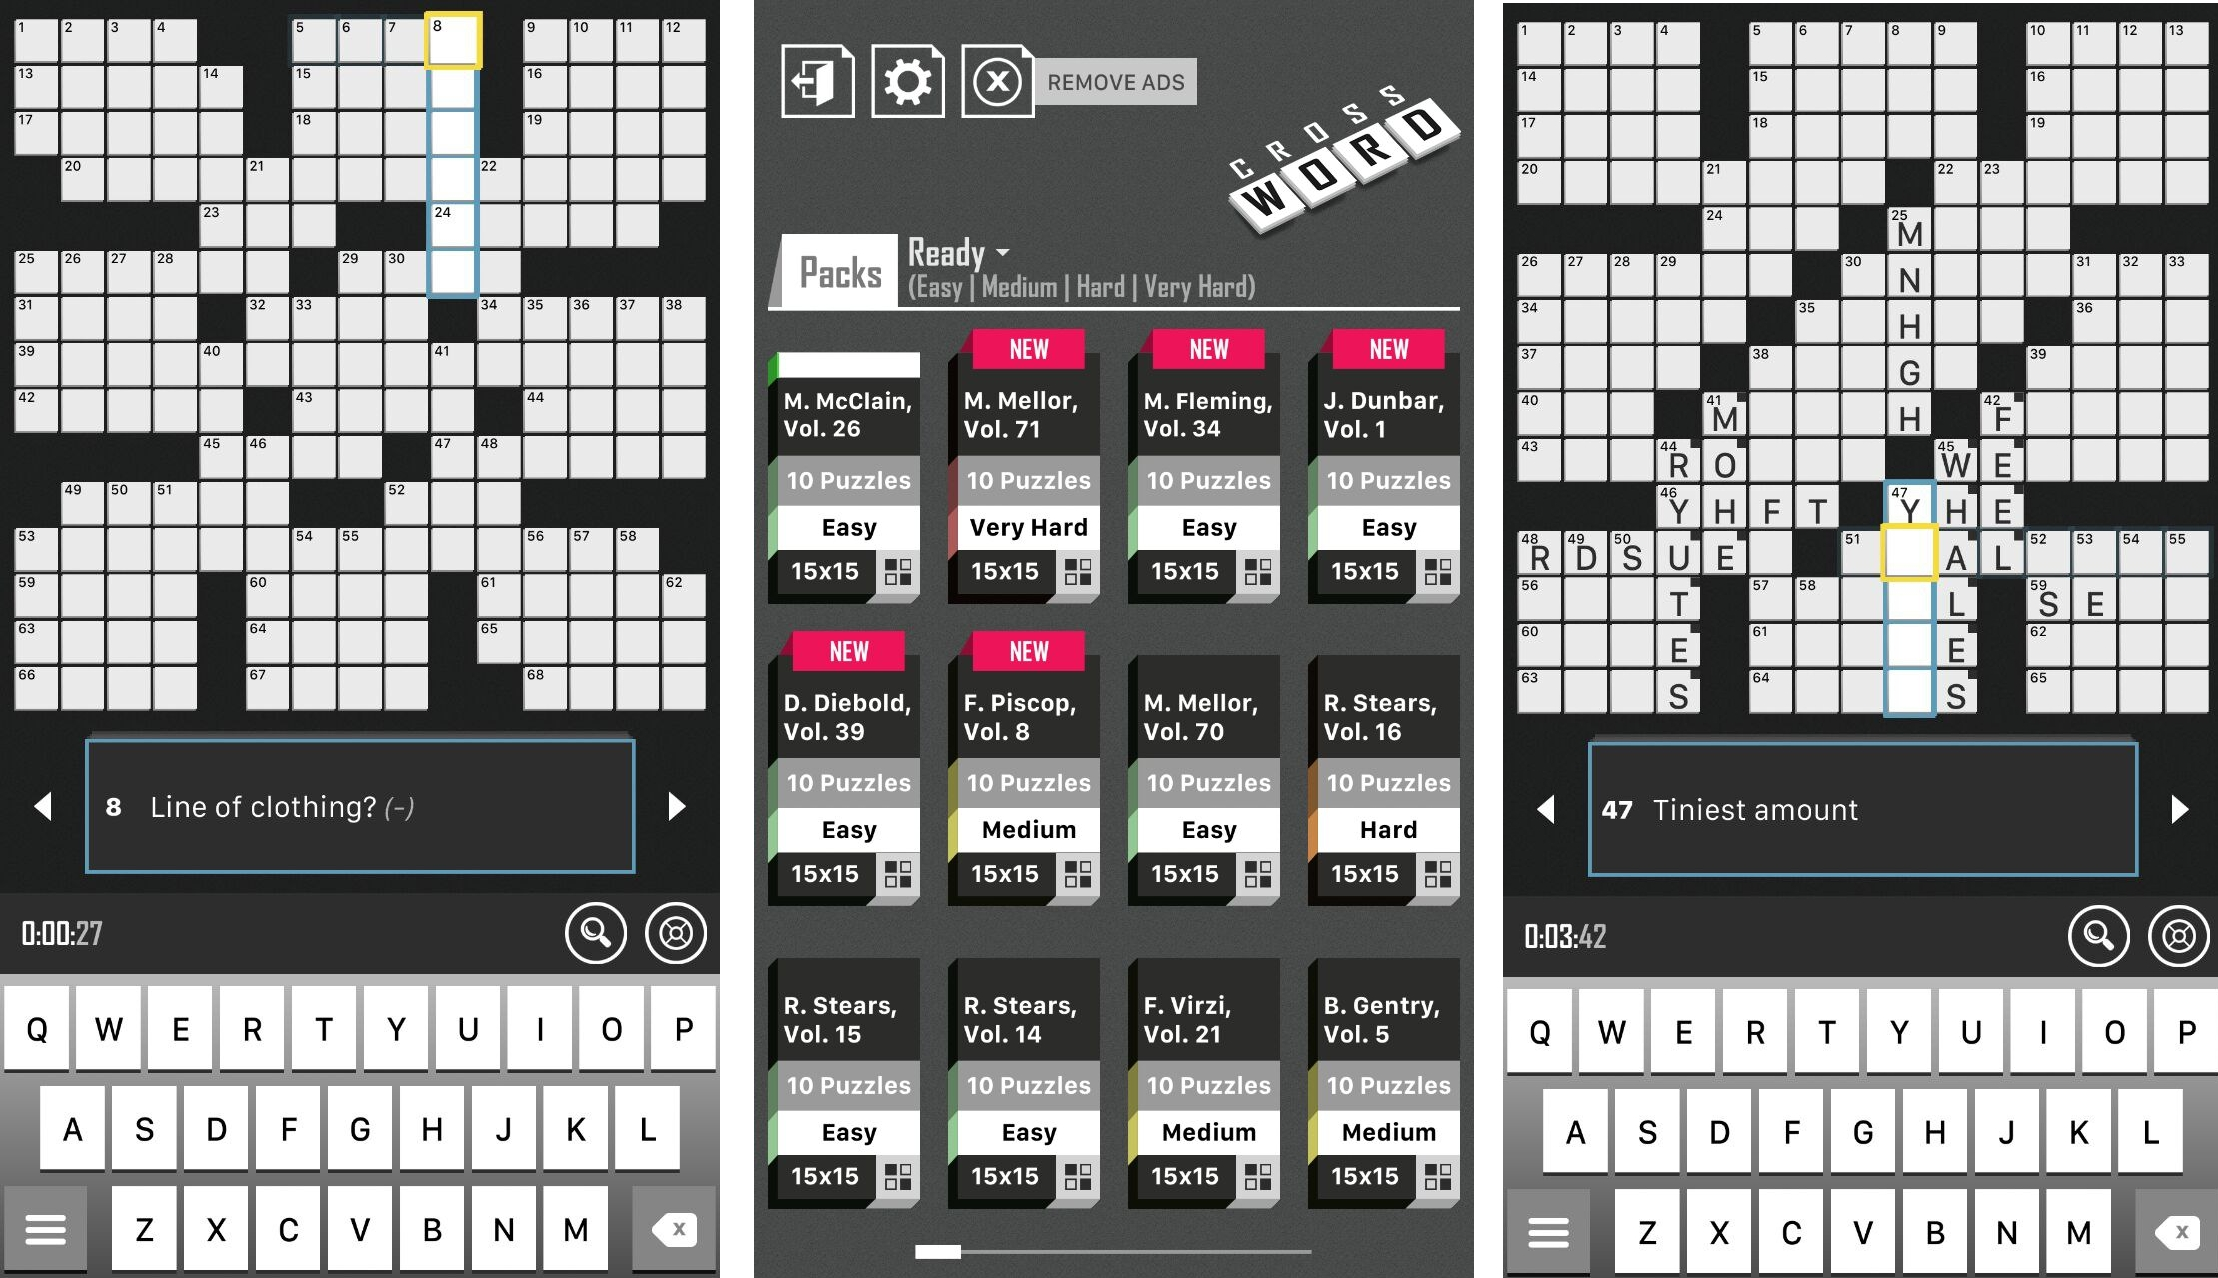
\includegraphics[width=0.9\textwidth]{Figuras/crosswordPuzzleFree.jpg}
    
    Fonte: Elaborada pelo autor
\end{figure}

\item[Crossword Quiz]\footnote{\url{https://play.google.com/store/apps/details?id=com.randomlogicgames.crossword&hl=pt_BR}} \hfill \\
Crossword Quiz (\autoref{fig:crossQuiz}) é um aplicativo de palavras cruzadas com uma abordagem mais fácil por não disponibilizar todas as letras do teclado, tornando a resposta mais fácil para o usuário. Além disso, o aplicativo não conta apenas com dicas escritas, mas inclui imagens. As funcionalidade que se destacam são: (i) Não mostrar todo o teclado, apenas algumas letras; (ii) Mostra imagens como dicas além de textos; (iii) Tutorial inicial intuitivo e completo.

\begin{figure}[H]
\centering
    \caption{Telas do aplicativo \textit{Crossword Quiz}}
    \label{fig:crossQuiz}
    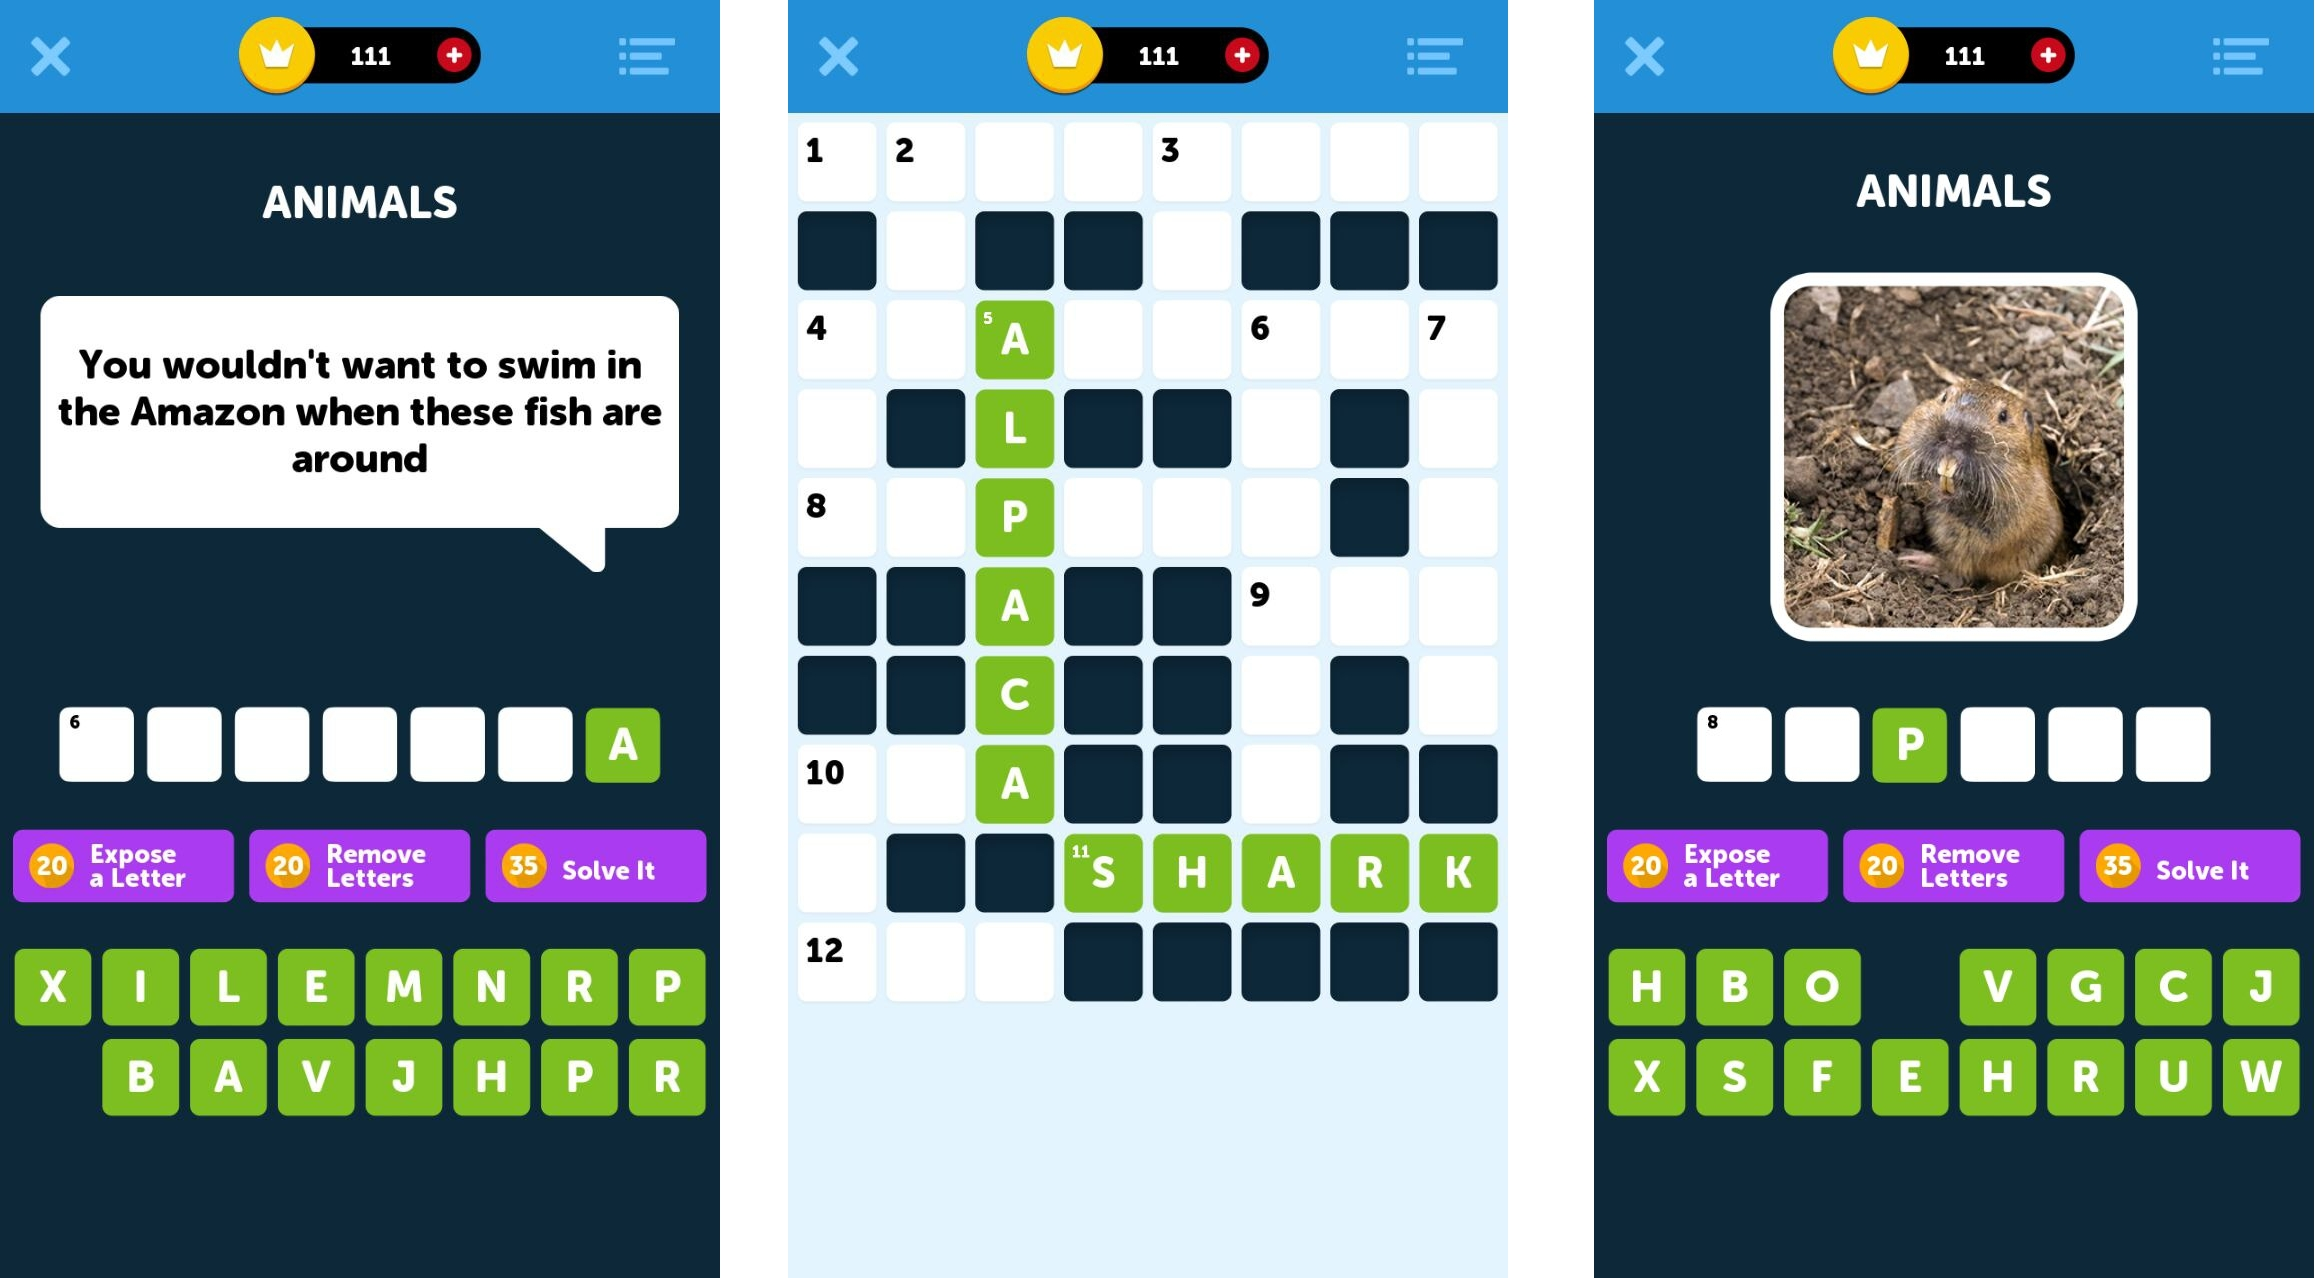
\includegraphics[width=0.9\textwidth]{Figuras/crosswordQuiz.jpg}
    
    Fonte: Elaborada pelo autor
\end{figure}

% inicio n deixe a vovó cair

\item[Não deixe a vovó cair]\footnote{\url{https://play.google.com/store/apps/details?id=com.GazGames.SalveVovo&hl=pt_BR}} \hfill \\
Não deixe a vovó cair (\autoref{fig:nDeixeVovoCair}) é um aplicativo que visa reduzir os riscos do ambiente domiciliar. Produzido pelo Centro de Telessaúde do Hospital das Clínicas – UFMG e pela Rede de Teleassistência de Minas Gerais, possui 4 níveis que representam áreas de uma casa: Banheiro, Quarto, Cozinha e Sala. Além disso, conta com a ajuda do cão Neca que representa o cachorro da dona e guia o usuário nos passos do jogo.
\begin{figure}[H]
\centering
    \caption{Telas do aplicativo \textit{Crossword Quiz}}
    \label{fig:nDeixeVovoCair}
    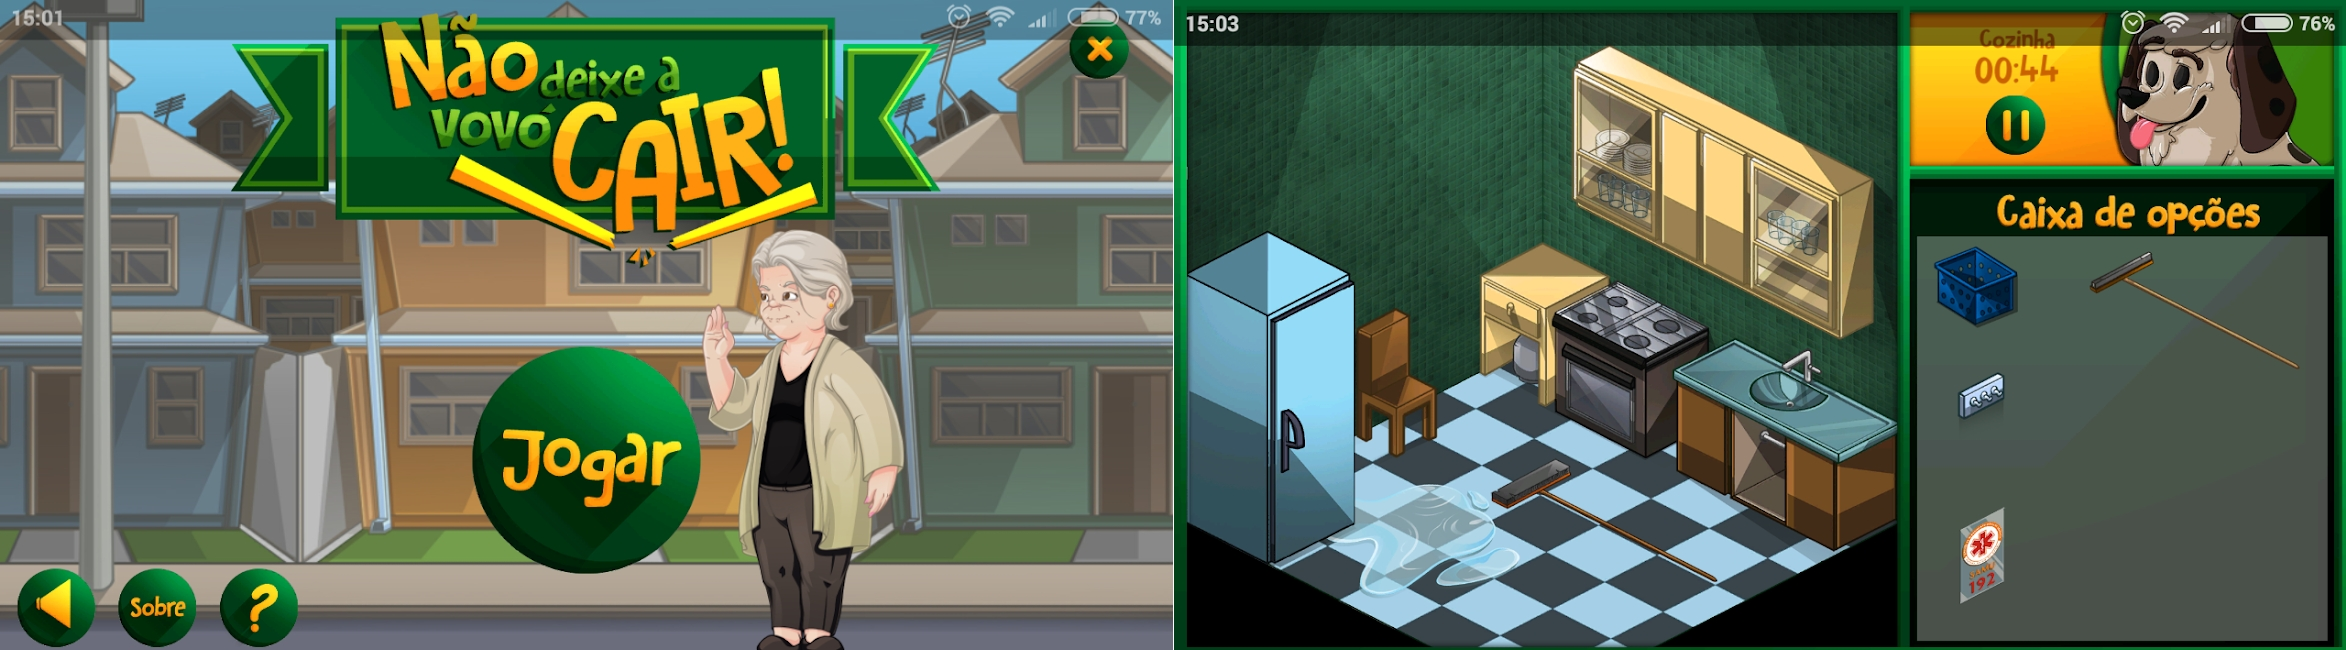
\includegraphics[width=0.9\textwidth]{Figuras/nDeixeVovoCair.jpg}
    
    Fonte: Elaborada pelo autor
\end{figure}

% fim

\end{description}


\begin{table}[!ht]
\centering
\caption{\textit{Funcionalidades das aplicações educacionais}}
\centering
\footnotesize
\begin{tabular}{p{6cm} p{10cm}}
\toprule
\textbf{Aplicativo} & \textbf{Funcionalidades}                                              \\ \midrule

Engaging congress   & \begin{tabular}[c]{@{}l@{}}Vídeos educativos\\ Perguntas relacionadas ao conteúdo\\ Nota após término dos exercícios\\ Botões de dúvida em todas as telas\end{tabular}                                                                 \\ \midrule
Play PBS KIDS Games & \begin{tabular}[c]{@{}l@{}}Funcionamento offline\\ Gerenciamento de consumo de memória\\ Obtenção de detalhes de desenhos passados na TV PBS Kids\end{tabular}      \\ \midrule
Human Anatomy Atlas & \begin{tabular}[c]{@{}l@{}}Interatividade com estruturas 3D\\ Mais de 1000 questões para testes\\ Realidade aumentada\\ Sete idiomas disponíveis\end{tabular}    \\ \midrule
Bini Super ABC & \begin{tabular}[c]{@{}l@{}}Aprendizado das letras por sons\\ Reforço do material aprendido\\ Controle de responsáveis para jogos\end{tabular}                \\ \midrule
Crossword Puzzle Free & \begin{tabular}[c]{@{}l@{}}Teclado não nativo, utiliza um personalizado\\ Dica acima do teclado\\ Botão de dica para a palavra\end{tabular}                \\ \midrule
Crossword Quiz & \begin{tabular}[c]{@{}l@{}}Não mostra o teclado todo, apenas algumas letras\\ Mostra imagens em vez de dicas em texto também\\ Tutorial inicial mostrando todos os passos antes da primeira partida\end{tabular}                \\ \midrule
Não deixe a vovó cair & \begin{tabular}[c]{@{}l@{}}Tutorial inicial ensinando o uso do aplicativo\\ Dicas em meio ao jogo para aplicações reais \\ Marcação do tempo para desafiar o usuário a melhorar cada vez mais \end{tabular}                \\ \midrule
\end{tabular}
\label{tab:sprint}
Fonte: Elaborada pelo autor
\end{table}


\section{Estudos sobre Ensino voltado para idosos}

Um dos objetivos do projeto é desenvolver uma aplicação educacional voltada para o público idoso. Portanto, faz-se necessário analisar o contexto relacionado ao Ensino voltado ao público idoso, a fim de auxiliar no desenvolvimento do projeto. 
Como pode ser visto na seção \ref{sec:introd}, a expectativa de vida no mundo subiu, e em países em desenvolvimento como o Brasil esse cenário é intensificado com prospecções de quadruplicação de pessoas com 60 anos ou mais \citep{demografico2010disponivel}. Dessa maneira, surge um novo desafio: adequar as práticas educacionais a esse público. De acordo com \cite{rethinkingTeacherEducation}, a situação requer fatores  que não podem ser trabalhados sem a reconstrução da atual abordagem na educação. É necessária a mudança da direção de pensamento sobre o público idoso aliada à construção de métodos que possam auxiliá-los ou enriquecer pedagogicamente as ofertas de ensino.

Dentre as possibilidades de abordagem, há a educação continuada ou educação permanente, a qual objetiva capacitar um indivíduo após o período escolar ou ao longo da vida da pessoa. Assim, aplicada à área Gerontológica esse tipo de educação pode ser utilizada em iniciativas educacionais \citep{neri2001palavras}. 

\cite{zemke198430}, citam princípios que se relacionam a aprendizagem de adultos, os quais podem ser aplicados ao público idoso. Há a divisão em três principais questões: (i) motivações para aprender; (ii) desenho curricular; (iii) sala de aula. Há uma série de afirmações feitas pelos autores (Tabela \ref{tab:questoesAprIdosos}), que podem ser aplicadas ao ensino de idosos.

\begin{table}[!ht]
\centering
\caption{\textit{Questões que podem ser consideradas para o ensino-aprendizagem de idosos}}
\centering
\footnotesize
\begin{tabular}{p{5cm} p{5cm} p{5cm}}
\toprule
\textbf{Quanto às
motivações para aprender} & \textbf{Quanto ao
desenho curricular} & \textbf{Quanto à
sala de aula}                                   
\\ \midrule

Eventos específicos de mudanças de
vida (casamento, divórcio, aposentadoria, dentre outros) fazem com que
os adultos busquem experiências de
aprendizagem.
& 
Alunos adultos e idosos tendem a
preferir cursos práticos a cursos teóricos e conceituais.
&
Aulas expositivas e longas aumentam a taxa de irritação.
\\ \midrule

Quanto maior o número de eventos
de mudanças de vida, mais probabilidade de buscar esta experiência.
& 
Informações conflitantes àquelas
consideradas verdadeiras pelos adultos e idosos são integradas de maneira mais lenta.
&
Idosos trazem uma grande experiência de vida para a sala de aula e
esta vantagem deve ser reconhecida,
extraída e usada.
\\ \midrule

Os adultos (e idosos) acreditam que
terão uso do conhecimento ou habilidade adquirida, de maneira que
buscam aplicar e seguir aquilo que
aprenderam.
& 
Tarefas de passos rápidos, complexas e incomuns interferem na aprendizagem e entendimento.
&
Novos conhecimentos devem ser integrados aos conhecimentos prévios
do aluno.
\\ \midrule

O aumento ou manutenção da autoestima e prazer também são consideradas motivações para o ato de
aprender.
& 
Por serem mais lentos em algumas
tarefas de aprendizagem psicomotoras procuram não realizar tentativas e evitam errar, tendendo a uma
maior precisão nas tarefas.
&
O instrutor deve saber equilibrar os
conteúdos com as experiências relevantes dos alunos e o tempo de aula.
\\ \midrule


& 
É necessário que o desenho curricular seja baseado em conceitos e
ideias que estejam em concordância
com os educandos.
&
Integração de novos conhecimentos
e habilidades requerem um maior
tempo de transição e esforços.
\\ \midrule
\end{tabular}
\label{tab:questoesAprIdosos}

Fonte: \cite{Oliveira2019_quali}
\end{table}

As principais dificuldades sofridas pelo público idoso são \citep{euromed}:

\begin{itemize}
    \item Problemas em absorver novas informações
    \item Crescente dificuldade de compreender frases complexas de acordo com a idade
    \item Esforço para entender inferências
    \item Dificuldades de audição
    \item Problemas de coordenação motora
    \item Perda crescente de visão
\end{itemize}

Tendo em vista tais dificuldades, faz-se necessária sua consideração no desenvolvimento do aplicativo, objetivando uma maior efetividade na compreensão do conteúdo pedagógico por parte do usuário idoso.

Ademais, é imprescindível citar a interferência das emoções no processo de aprendizado. A impaciência, relacionada a negatividade emocional associada a usuários os quais possuem dificuldades de aprender novas habilidades, é um fator que torna seu aprendizado ainda mais dificultoso \citep{Edukacja}. Portanto, proporcionar um ambiente emocionalmente saudável bem como sensações emocionais positivas motivantes, torna-se imperioso para possibilitar um melhor rendimento por parte do usuário idoso que estuda o assunto.

Outro fator importante a ser considerado no ensino ao público idoso é a perda de memória. A informação adquirida por meio da visão é mais facilmente esquecida que a ouvida; por consequência,  faz-se necessária a adoção de conteúdo auditivo nos métodos de ensino. Concomitantemente ao material auditivo, é recomendada a repetição frequente do conteúdo a fim de reduzir a taxa de esquecimento e elevar o nível de retenção do usuário idoso \citep{euromed}.

Segundo \cite{Edukacja}, trabalhar em pequenos grupos é a maneira mais efetiva quando se trata de atividades educacionais para idosos. Isso ocorre pois há uma rejeição aos métodos tradicionais de trabalho, pois esperam um tipo de educação baseada em relações pessoais, a qual é mais fácil de ser aplicada em pequenos grupos. Assim, é recomendado o uso do aplicativo desenvolvido em grupos de alunos idosos, uma vez que elevariam a proximidade entre os usuários, beneficiando o aprendizado.

Nesta seção puderam ser analisados diversos aspectos os quais devem ser observados no processo de ensino aos idosos. Desde incentivos indiretos para a motivação, até a preocupação direta com a repetição de conteúdo a fim de diminuir a taxa de esquecimento. 

\section{Estudo sobre os artefatos}
Com o intuito de auxiliar a elicitação de requisitos para o desenvolvimento do aplicativo, mostrou-se necessário o estudo de artefatos.
Assim, tal estudo será tratado com maiores detalhes sobre as diretrizes de acessibilidade WCAG 2.1 e os padrões pedagógicos do ReqML-Catalog \citep{soad2017reqml}.

\subsection{Pesquisa sobre recomendações da WCAG 2.1}
A fim de proporcionar uma experiência de uso do aplicativo respeitando as limitações do usuário, foram analisadas as diretrizes de acessibilidade contidas na \textit{Web Content Accessibility Guidelines} \citep{wcag}. Ela é um conjunto de recomendações criadas pela
\textit{World Wide Web Consortium} \citep{w3c} com o objetivo de tornar o conteúdo da Web mais acessível para pessoas com deficiências tais como: cegueira ou baixa visão, surdez ou indivíduos com perda de audição, pessoas com limitações de movimentação, deficiências de fala, fotossensibilidade e limitações cognitivas. As recomendações abrangem \textit{desktops}, \textit{notebooks}, \textit{tablets} e dispositivos móveis, os quais são o foco desse projeto. É importante destacar que a versão 2.1 foi construída respeitando a versão 2.0, publicada em dezembro de 2008. O documento foi revisado pelos membros da W3C, desenvolvedores de software e por outros grupos interessados, os quais foram julgados capazes pela própria W3C. Os 4 princípios utilizados para a acessibilidade na Web são: perceptível, operável, compreensível e robusto.
\begin{itemize}
    \item Perceptível - Informações e componentes de interface do usuário precisam ser apresentadas de maneira que ele perceba
    \item Operável - Componentes da interface do usuário e navegação precisam ser operáveis
    \item Compreensível - Informações e as operações da interface do usuário devem ser compreensíveis
    \item Robusto - O conteúdo deverá ser robusto o suficiente para ser interpretado por uma variedade de agentes de uso, incluindo tecnologias de assistência
\end{itemize}

O WCAG possui três níveis de conformidade:
\begin{enumerate}
    \item Nível A: Pouco impacto no design
    \item Nível AA: Médio impacto no design
    \item Nível AAA: Muito impacto no design
\end{enumerate}

Embora a documentação oficial restrinja a aplicação dos níveis de conforidade a páginas web, ela ainda se mostrou importante para basear o impacto no design das telas do aplicativo. 
Serão destacados os critérios que mais influenciaram o desenvolvimento do aplicativo:

\begin{itemize}
    \item 1.2.2 Legendas (Nível A): Será disponibilizada a transcrição dos áudios e vídeos utilizados pelo aplicativo.
    \item 1.2.8 Mídias alternativas (Nível AAA): Além de ser disponibilizado o conteúdo em texto, também será oferecida a possibilidade de consumir o conteúdo em áudio ou vídeo.
    \item 1.4.3 Contraste mínimo (Nível AA): Serão respeitados os limites de contraste mínimo entre cores de 4.5:1.
\end{itemize}


\subsection{ReqML-Catalog}
Concomitantemente à WCAG 2.1, foi considerado o \textit{ReqML-Catalog}
\citep{soad2017reqml}, o qual se trata de um catálogo de requisitos para Aplicações Educacionais Móveis. Ele foi proposto com o objetivo de propiciar um maior apoio na formulação de requisitos para aplicativos de educação, visto que muitos ainda possuem problemas e desafios a serem resolvidos. Além disso, de acordo com a pesquisa feita pelos autores, não havia um conjunto de requisitos completos e bem definidos para Aplicações Educacionais Móveis. É importante destacar que a última versão é uma evolução de outras anteriormente produzidas, as quais foram desenvolvidas a partir de literatura sistemática, revisões, e baseadas no conhecimento de especialistas do assunto. 
O \textit{ReqML-Catalog} possui uma estrutura hierárquica de três níveis: \textbf{Pedagógico}, \textbf{Social} e \textbf{Técnico}, como se pode ver na Figura \ref{fig:reqML}.

\begin{figure}[H]
\centering
    \caption{ReqML-Catalog}
    \label{fig:reqML}
    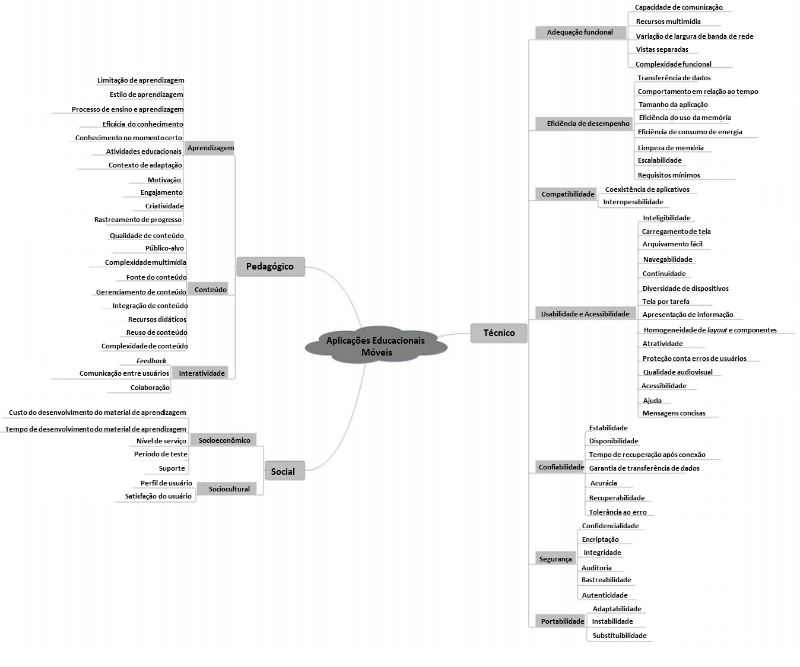
\includegraphics[width=0.9\textwidth]{Figuras/reqML-catalog.png}
    
    Fonte: \cite{soad2017reqml}
\end{figure}

As áreas que mais aproveitadas foram a Técnica e Social. Houve um maior destaque da área Pedagógica por dois motivos principais: (i) forneceu um panorama mais aprofundado de elementos essenciais para a educação obtidos de especialistas e literaturas especializadas; (ii) uma vez que o foco do projeto é auxiliar a educação, mais atenção precisou ser voltada à esta área.

\section{Levantamento e estudo dos conceitos e tecnologias para desenvolvimento de aplicações móveis}

Com o objetivo de desenvolver um aplicativo que possibilite o ensino a idosos, foi necessário compreender conceitos de Engenharia de Software (Requisitos), bem como a aprendizagem de tecnologias que permitissem a construção do código do mesmo. Dessa forma, serão investigados os principais conceitos relacionados ao desenvolvimento de aplicações móveis: 

\begin{itemize}
    \item Scrum, que trata sobre a metodologia de desenvolvimento adotada neste projeto;
    \item Requisitos;
    \item React Native, o qual contempla o levantamento e pesquisa da tecnologia adotada para concepção do sistema;
    \item UI/UX, que discute o conhecimento relacionado a interface e experiência do usuário.
\end{itemize}

\subsubsection{Estudos sobre Scrum e Requisitos} 
Para este projeto, decidiu-se adotar a metodologia de desenvolvimento ágil de software denominada \textit{Scrum}, uma vez que o produto final poderia sofrer com mudanças de requisitos por parte dos usuários. Essa metodologia foi concebida em 2001, com um grupo de 17 pessoas que se reuniu para discutir a respeito de desenvolvimentos mais leves de software, pois acreditavam que os modelos em voga eram lentos e burocráticos. O resultado foi o Manifesto Ágil \citep{agileManifesto}, em que os participantes propuseram princípios a serem seguidos. Segundo os criadores, deveria haver a valorização de: (i) Indivíduos e interações mais que processos e ferramentas; (ii) Software em funcionamento mais que documentação abrangente; (iii) Colaboração com o cliente mais que negociação de contratos; (iv) Responder a mudanças mais que seguir um plano.

Dentre os artefatos do \textit{Scrum}, devem ser citados o \textit{Product Backlog} e o \textit{Sprint Backlog}. O \textit{Product Backlog} possui todas as funcionalidades necessárias para o funcionamento do produto, as quais são ordenadas por prioridade. Já o \textit{Sprint Backlog} reúne as funcionalidades que serão desenvolvidas na atual \textit{Sprint} em execução.

Os eventos do Scrum são: (i) Sprint; (ii) Reunião de Planejamento da Sprint; (iii) Reunião Diária; (iv) Revisão da Sprint; (v) Retrospectiva da Sprint.

A \textbf{\textit{Sprint}} é essencial para o Scrum, durante um período de 2 a 4 semanas são desenvolvidas as atividades do \textit{Sprint Backlog}, as quais foram previamente selecionadas do \textit{Product Backlog}. Estas atividades são escolhidas na \textbf{Reunião de planejamento da \textit{Sprint}}. É importante destacar que concomitantemente à Sprint são realizadas \textbf{Reuniões diárias}, que possuem o objetivo de reunir o time de desenvolvimento a fim de sincronizar as atividades e criar um plano para as próximas 24 horas. Ao final do período separado para o incremento do produto, ocorre a \textbf{Revisão da Sprint}, com o objetivo de discutir o que foi feito, inspecionar o incremento e adaptar o \textit{Product Backlog}. A \textbf{Retrospectiva da Sprint} ocorre depois da Revisão da Sprint e antes da Reunião de planejamento da próxima Sprint, e é a oportunidade para o Time Scrum inspecionar a si próprio criar um plano para melhorias a serem aplicadas na próxima Sprint.

Ademais, existem funções diferentes para os membros chamadas de papéis. São eles: \textit{Product Owner}; Time de Desenvolvimento e \textit{Scrum Master}. 
O \textit{Product Owner}, ou dono do produto, se encarrega de maximizar o valor do produto e gerenciar os \textit{Backlogs}. O Time de Desenvolvimento concentra os profissionais responsáveis pelos incrementos do produto. Por fim, o \textit{Scrum Master} orquestra toda a equipe e deve garantir que o Scrum seja entendido e aplicado.

Outro fator importante para o desenvolvimento de um software são os requisitos. De acordo com \cite{Sommervile2010}, eles podem ser definidos como os serviços que o sistema promove, as restrições de operação e as descrições do que o sistema deveria realizar. É importante destacar a Engenharia de Requisitos, a qual fornece mecanismos apropriados para o entendimento da demanda do consumidor, análise de suas necessidades, avaliação da viabilidade, negociação de uma solução, especificação de uma solução não ambígua, validação da especificação e gerenciamento de requisitos enquanto são transformados em um sistema operacional \citep{Pressman2014}. 

Três são os principais tipos de requisitos \citep{Sommervile2010}:
\begin{itemize}
    \item \textbf{Requisitos funcionais}: são declarações de serviços que o sistema deve prover, como o sistema deve reagir a determinados tipos de entrada, e como deveria funcionar em situações particulares. Em alguns casos, os requisitos funcionais podem também explicitar o que o sistema não deveria fazer.
    
    \item \textbf{Requisitos não funcionais}: são restrições dos serviços ou funções oferecidos pelo produto. Incluem restrições de tempo, de processos de desenvolvimento, e restrições impostas por padrões. Requisitos não funcionais frequentemente se aplicam ao sistema como um todo, em vez de se aplicar a serviços ou \textit{features} individuais.
    
    \item \textbf{Requisitos de domínio}: são derivados do domínio de aplicação do sistema, e não de necessidades específicas de usuários do sistema. Podem ser novos requisitos funcionais, restringindo os já existentes. 
\end{itemize}


\subsection{Estudos sobre React Native} 
Há diversas maneiras de desenvolver um aplicativo móvel. O modo convencional é utilizar a linguagem nativa: Java (Android) e Swift/Object-C (iOS), todavia isso causa o empecilho de se disponibilizar o aplicativo apenas para uma plataforma. Ainda, é possível usar \textit{frameworks} híbridos que recorrem ao uso de \textit{web-views} para renderizar a aplicação e disponibilizar para os dois sistemas operacionais, pode-se citar Ionic, Titanium, e PhoneGap. Entretanto, o desempenho de aplicativos construídos com tais tecnologias é precário. Pensando no problema, durante a conferência do React.js em 2015, o Facebook introduziu seu novo \textit{framework} React Native, o qual prometia revolucionar a maneira de desenvolver aplicativos móveis. A premissa era simples, possibilitar o desenvolvimento \textit{mobile} sem a necessidade de programação diferente para os dois sistemas operacionais líderes.

Levando isso em conta, as principais vantagens e desvantagens do \textit{framework} serão listadas a seguir na Tabela \ref{tab:vanDesvRN}:

% Vantagens e desvantagens
\begin{table}[!ht]
\centering
\caption{\textit{Vantagens e desvantagens do React Native}}
\centering
\footnotesize
\begin{tabular}{p{7cm} p{7cm}}
\toprule
\textbf{Vantagens} \citep{danielsson2016} & \textbf{Desvantagens}                          
\\ \midrule
O desenvolvimento ocorre em uma única linguagem, sendo possível utilizar o aplicativo em iOS ou Android.
& 
Incerteza da possibilidade de executar frequentes tarefas em segundo plano quando o aplicativo já está sendo executado em segundo plano \citep{sodebergJohansson}.
\\ \midrule

A documentação oficial dá grande suporte e ajuda.
& 
Testes concluem que a frequência GPU, carregamento de CPU, uso de memória e consumo de energia são levemente inferiores ao desenvolvimento nativo \citep{danielsson2016}.
\\ \midrule

O \textit{React Native} não possui nenhum efeito negativo na experiência do usuário, pois a diferença de desempenho é imperceptível para a grande maioria dos usuários.
& 

\\ \midrule

\end{tabular}
\label{tab:vanDesvRN}

Fonte: Elaborada pelo autor
\end{table}

Embora existam algumas desvantagens do uso do React Native, em termos gerais é uma excelente alternativa para o projeto, pois não compromete de maneira significante a performance do aplicativo. Além disso possibilita o uso nas plataformas iOS e Android, alcançando assim, um número maior de usuários.

\subsection{Estudos sobre UI/UX}
Visando corroborar as boas práticas de desenvolvimento de aplicações móveis, é essencial a compreensão dos conceitos de Interface de Usuário bem como Experiência do Usuário. Sobretudo no desenvolvimento deste projeto, o qual possui o foco em usuários idosos.

Assim, pode-se dizer que a Interface de Usuário (UI) se refere a um sistema e um usuário interagindo um com outro por meio de comandos para operar o sistema, inserir dados, e usar o conteúdo \citep{joo2015}. Já a Experiência de Usuário (UX), segundo \cite{marc2008}, é uma perspectiva distinta da qualidade de tecnologia interativa. O autor ainda define UX como uma avaliação momentânea e primária da sensação (bom-ruim) enquanto interage com o produto ou serviço. Dessa forma, UX troca a atenção dos produtos e materiais para as sensações humanas - o lado subjetivo do uso do produto. Ainda, de acordo com \cite{castilla2017}, a UX representa uma mudança do próprio conceito de usabilidade, pois o objetivo não se reduz a melhorar a sensação do usuário na eficácia, eficiência e facilidade de aprendizagem, mas sim tentar resolver o problema estratégico da utilidade do produto para o usuário. 

Dessa maneira, pode-se concluir que a interface e experiência do usuário cumprem papéis essenciais no desenvolvimento de um produto, sendo indispensável seu planejamento. Ainda, tendo em vista o público alvo do atual projeto, usuários idosos, torna-se necessária a atenção e cuidado no assunto a fim de alcançar os objetivos finais.

Portanto, tendo em mente os motivos acima citados, foi realizado um minicurso sobre a Experiência de usuário e Interface de usuário com uma especialista da área UI/UX cujo título era ``Como incluir UX e UI Design nos seus projetos''. \textbf{\textit{A realização se deu na 22ª Semana da Computação da Universidade de São Paulo, campus de São Carlos, no dia 03/10/2019}}. O minicurso se mostrou de grande importância, uma vez que possibilitou a expansão do conhecimento do assunto em termos práticos, sendo possível sua aplicação no projeto.

\section{Desenvolvimento}
Nesta seção, são abordados os aspectos relativos ao desenvolvimento do aplicativo móvel. Partindo de um protótipo inicial, analisando-se o algoritmo de geração de palavras cruzadas e finalmente sendo discutido o Produto Mínimo Viável (\textit{MVP}).

\subsection{Protótipo inicial}
% Ficou claro que esse prototipo e do doutorado de outra pessoa e estou continuando?

Este projeto tomou como base o trabalho realizado por \cite{oliveira2018crossword}. O referido trabalho desenvolveu, dentre outros resultados, um protótipo do aplicativo \textit{Crossword Learning}, o qual é classificado como uma aplicação educacional móvel e possui estrutura baseada nos perfis de usuários idosos. O objetivo era apoiar o ensino dos usuários sobre diversos assuntos com o suporte de palavras cruzadas.

É importante destacar que para a construção do protótipo foi realizada uma pesquisa, cujos dados foram coletados e analisados e serviram como base.
Utilizando-se um questionário com o objetivo de verificar o interesse dos idosos em aplicações educacionais móveis, 28 participantes com idade entre 50 e 81 anos colaboraram. Ainda, foi feita uma entrevista com dois especialistas no ensino desse público.

A validação da interface do aplicativo, cujo foco foi acessibilidade e usabilidade, foi feita com dez participantes e está servindo de base para a elaboração de requisitos. 

\subsection{Estudo do algoritmo de geração de palavras cruzadas}
Uma vez que o protótipo inicial só contemplava uma interface, o próximo passo era a determinação de um algoritmo que pudesse gerar um tabuleiro de palavras cruzadas. 

Assim, foi tomado como base o algoritmo feito em \textit{javascript} por \cite{layoutGenerator}, o qual foi modificado para atender as necessidades deste projeto. Ele funciona a partir de uma lista de palavras que serão usadas para construir um tabuleiro. Além disso, permite que o usuário escolha o tamanho do tabuleiro, e caso uma palavra seja grande demais e não consiga ser inserida, ela é eliminada da lista e não segue para os próximos passos. A seguir serão explicitados os detalhes do algoritmo.

O procedimento inicia gerando uma tabela com o mesmo número de colunas e linhas. Essa quantidade é definida multiplicando-se o tamanho da maior palavra por um fator definido como 3. Por exemplo, caso a maior palavra tenha 7 letras e o fator seja o mesmo 3, será gerada uma tabela 14x14. Isso ocorre para aumentar a probabilidade de interseção entre palavras. 

Após estas etapas, é iniciado o procedimento de inserção. É feita a tentativa de inserção para cada uma das palavras fornecidas em todas as posições possíveis do tabuleiro iniciando-se com a disposição horizontal e após a vertical. Caso ocorra algum conflito da palavra inserida com outra que já esteja no tabuleiro, a posição será ignorada. Uma vez terminada a tentativa de inserção de uma palavra em todas as posições, é feita a análise de pontuação entre elas. Apenas a posição que possuir a maior pontuação permanecerá. Para isso, são computados quatro tipos de pontuações, como mostrado na (\autoref{fig:codeScores}). As avaliações possuem os seguintes pesos percentuais:

\begin{itemize}
    \item Número de conexões - 70\%
    \item Distância do centro do tabuleiro - 15\%
    \item Vertical vs Horizontal - 10\%
    \item Tamanho da palavra - 5\%
\end{itemize}

\begin{figure}[H]
\centering
    \caption{Funções de avaliação de pontuações do tabuleiro}
    \label{fig:codeScores}
    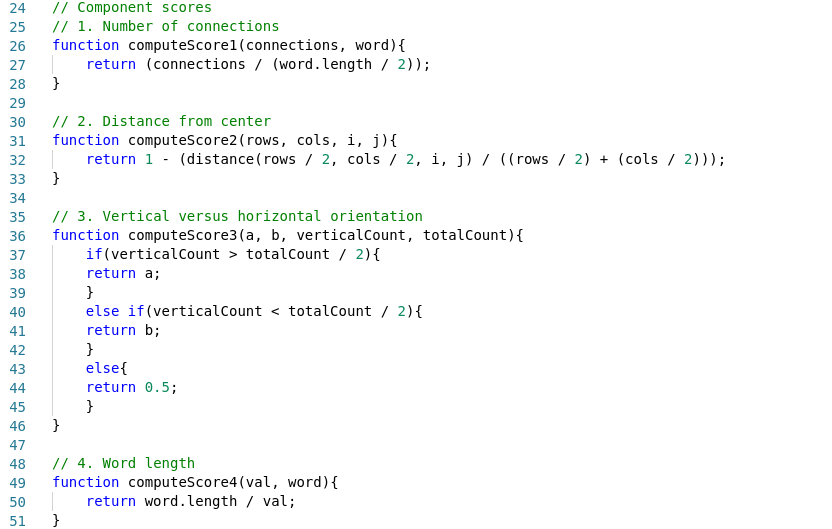
\includegraphics[width=0.9\textwidth]{Figuras/codeComponentScores.png}
    
    Fonte: \cite{layoutGenerator}
\end{figure}

O fator Vertical vs Horizontal tenta equilibrar a quantidade de palavras na horizontal e na vertical. Caso ocorra o caso de mais da metade das palavras já estar inseridas na horizontal e a palavra que está sendo analisada no momento estiver na vertical, ela é melhor avaliada.

Uma vez que a palavra é inserida armazena-se sua posição no tabuleiro, bem como sua orientação vertical ou horizontal e seu tamanho.

Esse processo é feito com todas as palavras da lista. Todavia, pode ocorrer o caso de uma palavra ficar isolada sem interseções, e portanto será eliminada. É importante lembrar que o tabuleiro está em um tamanho maior do que o desejado pelo usuário, pois no início ocorreu uma expansão das linhas e colunas ao multiplicá-las por um fator que havia sido definido como 3. Dessa maneira, restam colunas e linhas que estão vazias e podem ser eliminadas. Logo, o último passo é reduzir o tabuleiro para seu tamanho ideal respeitando o desejado pelo usuário. 

Como resultado final, o algoritmo exporta um arquivo \textit{JSON} (Figura \ref{fig:json}) contendo o tabuleiro de palavras cruzadas, nele há as palavras, suas orientações e as coordenadas de suas posições no tabuleiro.

\begin{figure}[H]
\centering
    \caption{Arquivo \textit{JSON} gerado como resultado final}
    \label{fig:json}
    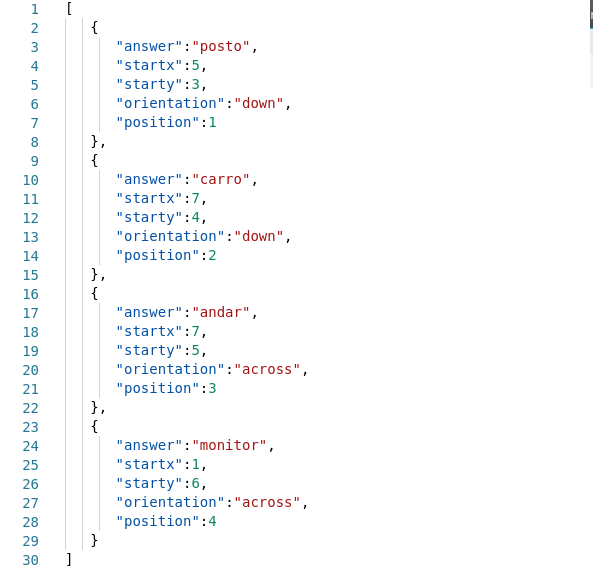
\includegraphics[width=0.9\textwidth]{Figuras/codeJSONresult.png}
    
    Fonte: Elaborada pelo autor
\end{figure}

\subsection{Desenvolvimento do Produto Mínimo Viável (\textit{MVP})}
% Escrever o que foi feito em termos de desenvolvimento técnico {
%     - Colocar algumas linhas de código
%     - Falar de alguns desafios do React Native
%     - Explicar a arquitetura do React Native do app
% }
Com o algoritmo descrito acima funcionando corretamente, foi possível construir um \textit{MVP}. Já que o desenvolvimento se deu utilizando o \cite{RN}, que permite a construção de aplicativos para Android e iOS, o processo se tornou ainda mais fácil pois a implementação do algoritmo supracitado foi feita em \textit{javascript}, a qual é a linguagem de programação também utilizada no \cite{RN}. Dessa maneira, a arquitetura do \textit{framework} se encarrega do processo que permite que o algoritmo seja executado no dispositivo móvel.

A tela de jogo foi desenvolvida da seguinte maneira: uma \textit{tag} \textit{<View>} comporta quatro \textit{tags} principais nativas do \textit{React Native}:

\begin{itemize}
    \item \textit{<FlatList>}, responsável por renderizar as células do tabuleiro
    \item \textit{<View>}, responsável por encapsular as também nativas \textit{tags} \textit{TouchableOpacity}. Em conjunto se tornam a seção que mostra a dica da resposta para a palavra selecionada 
    \item \textit{<View>}, que encapsula o componente customizado \textit{<Keyboard>}, o qual renderiza o teclado personalizado
    \item \textit{<Modal>}, que fica encarregada de expandir o texto quando o usuário realiza o toque na dica
\end{itemize}

A Figura \ref{fig:keyboard} mostra o componente \textit{<Keyboard>}. A linha 286 passa o um vetor contendo todas as letras pertencentes ao teclado personalizado para o componente. As linhas 287 e 288 passam as funções de inserção de letra e a função que faz a mudança de célula quando a letra é inserida. 

\begin{figure}[H]
\centering
    \caption{Trecho do código da \textit{<View>} que encapsula \textit{<Keyboard>}}
    \label{fig:keyboard}
    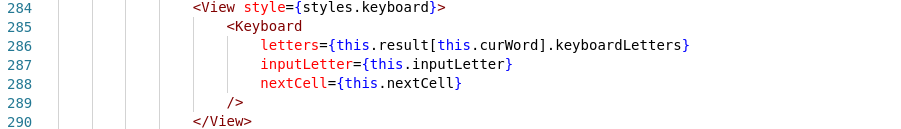
\includegraphics[width=1.0\textwidth]{Figuras/codeKeyboard.png}
    
    Fonte: Elaborada pelo autor
\end{figure}

O teclado personalizado foi introduzido por termos de acessibilidade, botões maiores permitem uma melhor experiência para o usuário idoso. É importante destacar que ele é formado pelas letras que compõem a palavra a ser preenchida acrescida de letras aleatórias.

\begin{figure}[H]
\centering
    \caption{Telas do MVP}
    \label{fig:mvp}
    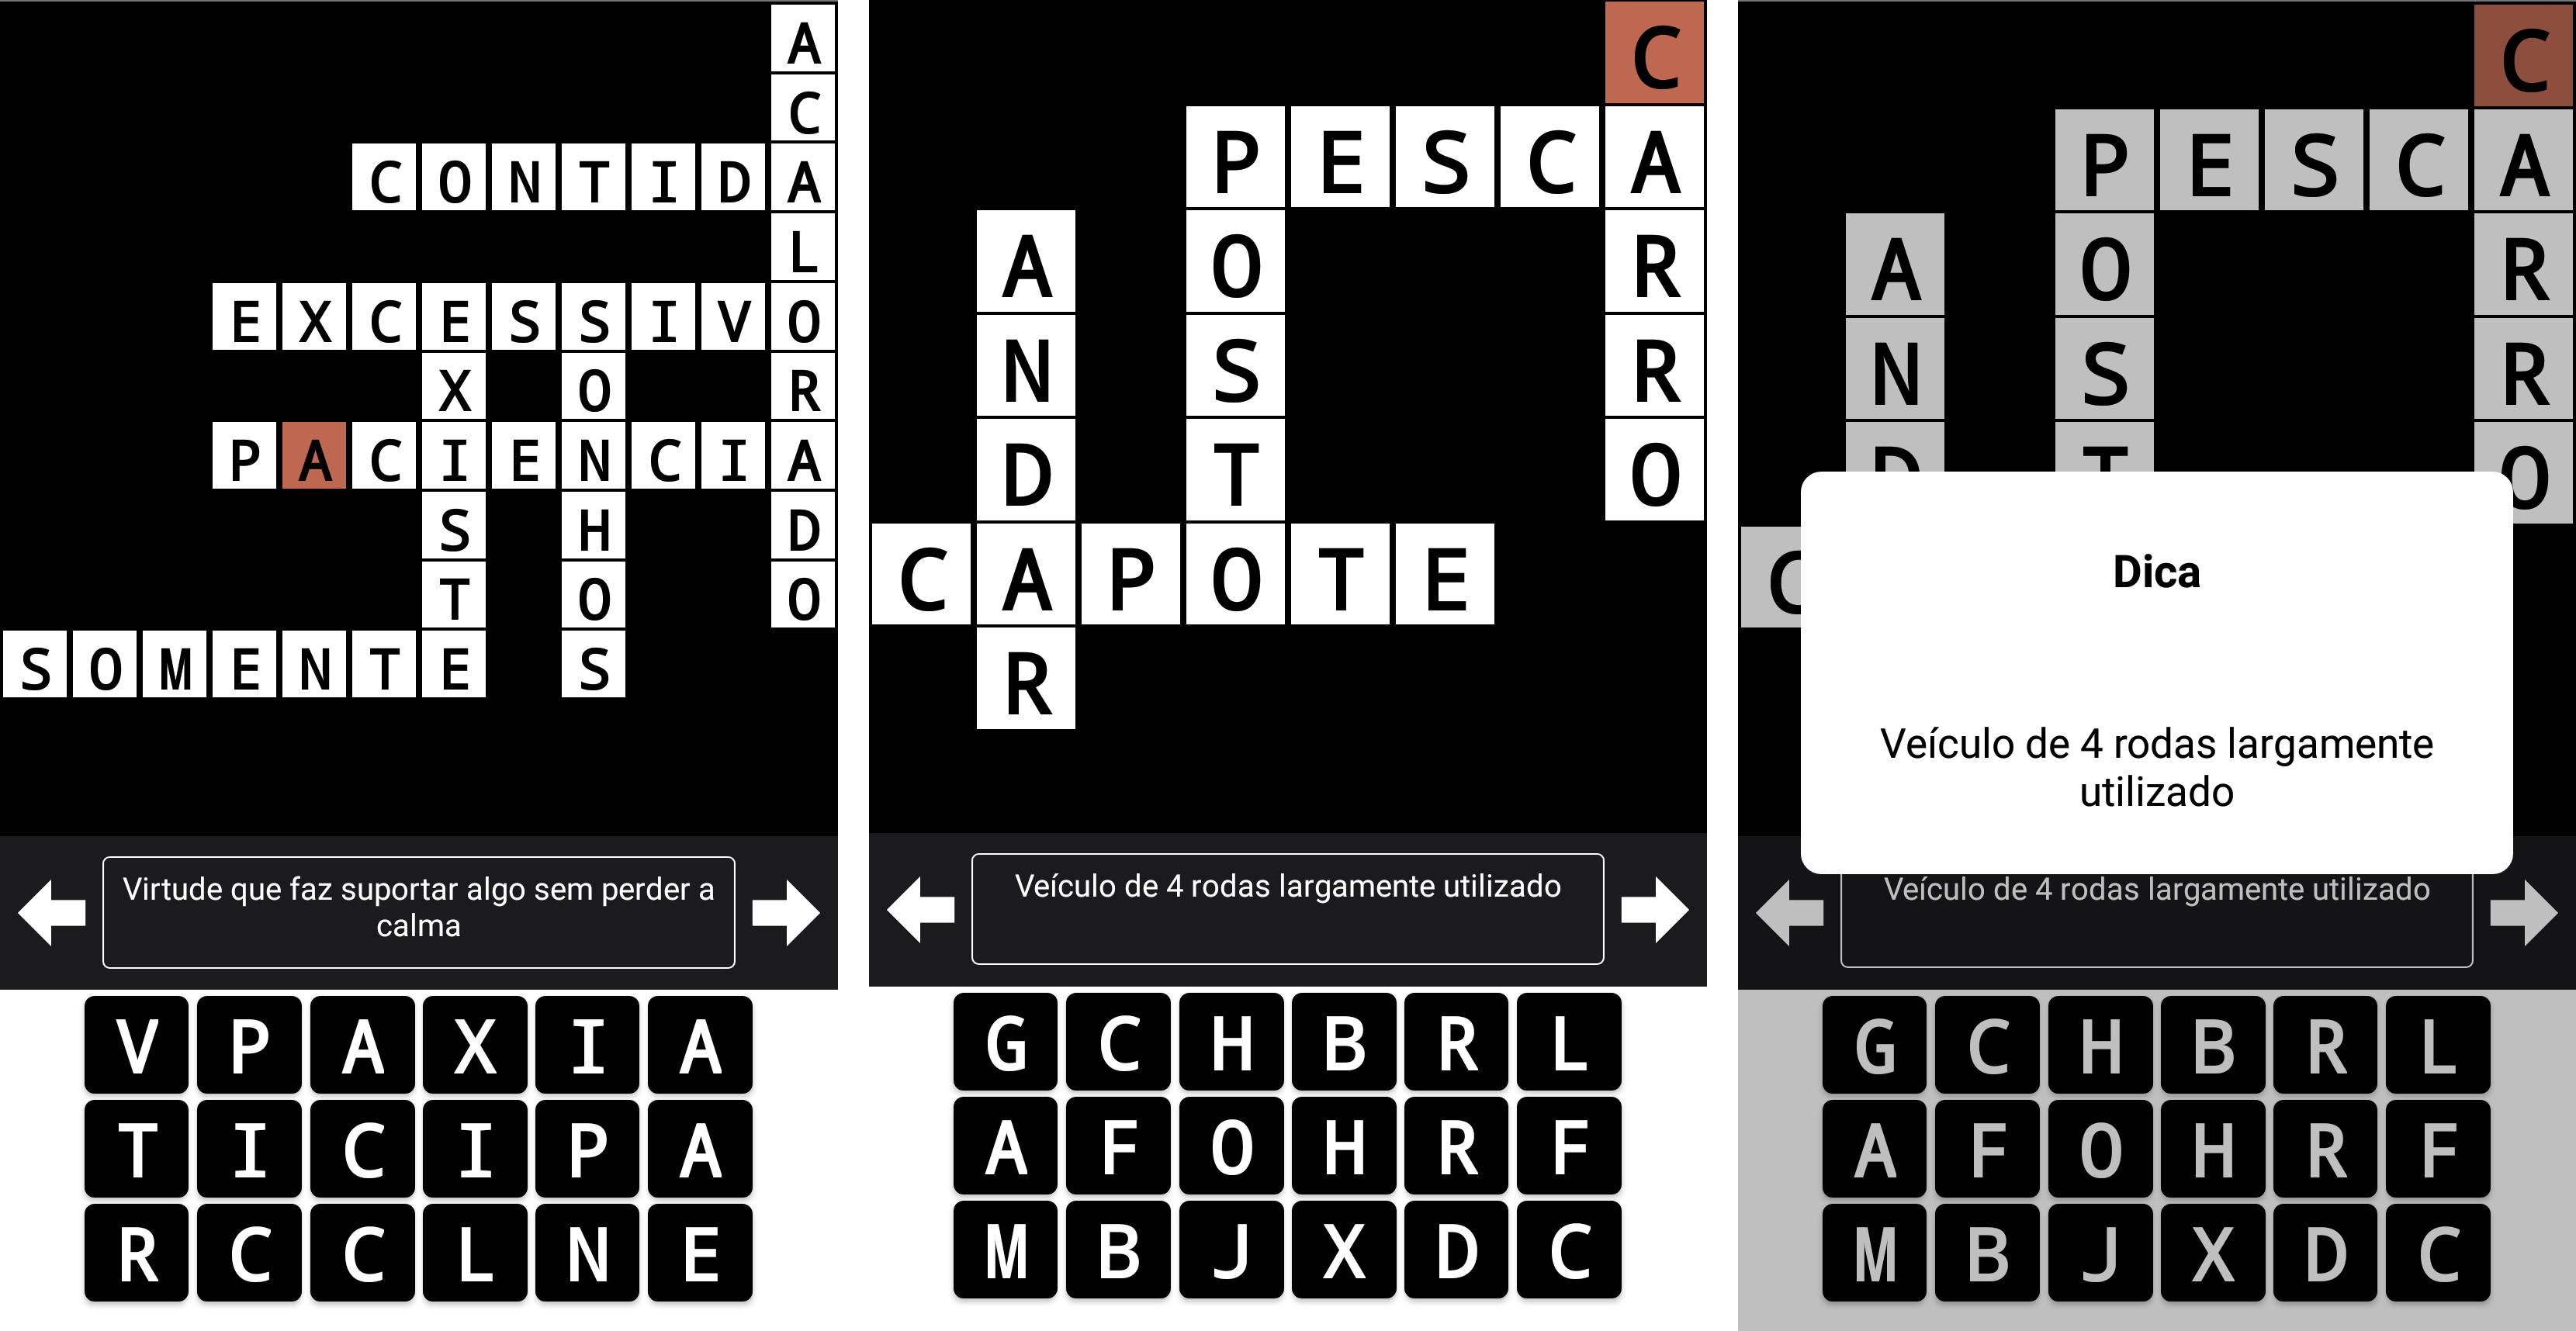
\includegraphics[width=1.0\textwidth]{Figuras/mvp.png}
    
    Fonte: Elaborada pelo autor
\end{figure}

Para algumas mudanças de informação na tela de jogo, decidiu-se utilizar a \textbf{Manipulação Direta} pois evita-se a renderização de toda a tela para pequenas mudanças, o que poderia acarretar problemas de desempenho. Dessa maneira, o estado dos componentes é modificado por meio de referência, acarretando em uma maior fluidez. Os elementos que recebem a Manipulação Direta são \textit{<Tiles>}, que são componentes customizados que renderizam as células do tabuleiro. 
% Ocorrem duas Manipulaçoes Diretas com esses componentes: alteração do foco e substituição da letra exibida.

Na Figura \ref{fig:codeDirectManipulation} pode-se observar uma função que faz uso da Manipulação Direta. \textit{inputLetter} recebe como argumento uma letra e promove a mudança do valor de uma propriedade no componente em que se faz a referência. Como cada célula do tabuleiro está armazenada em uma matriz, para acessá-la utiliza-se \textit{this.ref[posicaoI][posicaoJ]}. Nas linhas 208, 209 e 210 ocorre a mudança da propriedade \textit{text} usando a referência (\textit{.ref}) junto com o método \textit{setNativeProps}. Seu novo valor passará a ser o armazenado na variável \textit{letter}, a qual é recebida diretamente do teclado personalizado.

\begin{figure}[H]
\centering
    \caption{Método que utiliza manipulação direta}
    \label{fig:codeDirectManipulation}
    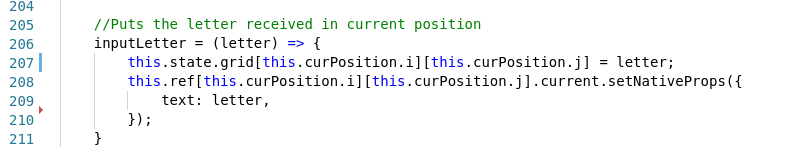
\includegraphics[width=0.9\textwidth]{Figuras/codeDirectManipulation.png}
    
    Fonte: Elaborada pelo autor
\end{figure}

% As mudanças de estado que ocorrem na tela de jogo são:

% \begin{itemize}
%     % informal por enquanto
%     \item substituição de letra no tabuleiro
%     \item mudança de cor para a célula que possui o foco
% \end{itemize}